\documentclass[11pt]{article}
\usepackage[table]{xcolor}
\usepackage{geometry}
 \geometry{
 a4paper,
 total={170mm,257mm},
 left=20mm,
 top=20mm,
 }
\usepackage{amsmath}
\usepackage{graphicx}

\usepackage{setspace}

\usepackage{amssymb}
\usepackage{epstopdf}
\usepackage{inputenc}

\usepackage{dashrule}
\usepackage{float}
\usepackage{hyperref}
\usepackage{url}
\usepackage{mwe}
\usepackage{caption}
\usepackage{longtable}
\usepackage{minted}
\usepackage{xr}


\usepackage[backend=biber,style=ieee]{biblatex}
\usepackage[toc]{appendix}
\usepackage[acronym]{glossaries}

\addbibresource{IndustrialProg.bib}

\hypersetup{ linktoc=all}
\graphicspath{ {./images/} }

\definecolor{light-gray}{gray}{0.95}
\newcommand{\code}[1]{\colorbox{light-gray}{\texttt{#1}}}

\begin{document}
\title{%
	\bf DocuTrace\\ 
    \large F20FC: Industrial Programming\\
    Coursework 2}

\author{
	Sam Fay-Hunt | \texttt{sf52@hw.ac.uk}
}

\maketitle
\thispagestyle{empty}
\pagebreak


\tableofcontents
\thispagestyle{empty}
\pagebreak


\setcounter{page}{1}

\section{Introduction}
The DocuTrace application is a moderate size, data-intensive application, its purpose is to analyse and display document tracking data from the website \href{https://issuu.com/}{issuu.com}. 
The website hosts a substantial number of documents, and provides anonymised usage statistics, the data is provided in the form of a sequence of individual JSON entries seperated by new lines. 


It is assumed the users of an application like DocuTrace would be someone with a high enough degree of technical competency to use simple Linux command line applications, the user would likely be a researcher (data science), or a business. 
The prior assumption leads to the assumption that the hardware running this application would be closer to server class than standard consumer hardware with higher CPU core counts and alot more RAM.
To try and compensate for the potential scale of the data a signifantly large amount of RAM is not mandatory to run this application, but a pool of aproximately 8GB of RAM should be installed on the system at a minimum when processing 3 million lines otherwise a performance penalty may be incurred.


DocuTrace was written in Python 3, it is intended to be run on Ubuntu 20.04, and has not been tested on other operating systems. 

\href{https://www2.macs.hw.ac.uk/~sf52/DocuTrace/html/index.html}{Comprehensive documentation} has been generated, a list of dependencies, installation and run instructions are provided, note the recommended entrypoint of the application is via the ``docutrace'' shell script, this script will automatically configure an environment variable to specify the output directory of graph files generated.

\subsection{Libraries}
\begin{itemize}
    \item numpy - Used for convienience and access to fast low-level vector operations.
    \item matplotlib - This library was used to display charts.
    \item user-agents - Helped translate the 'user-agent' JSON entry into a more readable format.
    \item pycountry - Converts countries alpha2 code into a full country name.
    \item pycountry-convert - Get the name of a continent for a given country.
    \item graphviz - Used to plot the "Also likes" graph.
    \item regex - This library is prefered to the standard "re" library because it has a full match method, and allows us to easily compile and reuse a regex expression.
    \item alive-progress - Provides beautiful, easy to implement progress bars when the total load time is unknown.
    \item python-decouple - Convieniently reads environment variables and .env files with no boilerplate code.
\end{itemize}


\section{Requirements Checklist}
% ------------------------------------------- REQUIREMENTS ---------------------------------------------------------------
\noindent{\Large \emph{The priority for each requirement is encoded as follows:}}

\begin{itemize}
    \item \textbf{Essential} - This priority indicates that this requirement must be implemented to satisfy basic functionality of the application, these requirements are all explicitly requested in the task brief.
    \item High - A high priority indicates that this requirement is important for providing a good quality application.
    \item Medium - A medium priority requirement is nice to have but if it is missing it is acceptable.
    \item Low - Low priority indicates that this is unlikely to be fulfilled, or it is generally unimportant for the applications functionality as a whole.
\end{itemize}

\begin{center}
    \begin{longtable}{|p{3cm}|p{7cm}|l|p{2cm}|}
        \hline
        \textbf{Requirement} & \textbf{Description} & \textbf{Priority} & \textbf{Status}\\
        \hline \endhead
        Runs on Linux & The application needs to run on an up-to-date Linux platform (Ubuntu 20.04) & \textbf{Essential} & Complete \\
        \hline
        Use Python 3 & The core logic of the application should be implemented in Python 3 & \textbf{Essential} & Complete\\
        \hline
        Views by country & Given a document UUID find from which countries the document has been viewed, display as histogram & \textbf{Essential} & Complete\\
        \hline
        Views by continent & Given a document UUID find from which continent the document has been viewed, display as histogram & \textbf{Essential} & Complete\\ 
        \hline
        Views by browser & For an input file count the number of occurrences for each browser used to access each document in the file, display full and truncated strings as histogram & \textbf{Essential} & Complete \\
        \hline
        Reader profiles & For each user find the total time spent reading documents, display the top 10 & \textbf{Essential} & Complete \\
        \hline
        Readers of document & For a given document identify all visitor UUIDs of readers of that document & \textbf{Essential} & Complete \\
        \hline
        Documents from reader & For a given reader identify all documents that reader has read & \textbf{Essential} & Complete \\
        \hline
        "Also likes" functionality & Using the readers of document and document from reader functionality return a list of documents sorted by a given sorting function as a parameter & \textbf{Essential} & Complete \\ 
        \hline
        "Also likes" graph & generate a graph that visualises the "Also likes" functionality & \textbf{Essential} & Complete \\
        \hline
        Simple GUI & Develop a simple GUI based on tkinter to display the statistical data and recieve input parameters & \textbf{Essential} & Complete \\
        \hline
        Command-line usage & Provide a command line usage to test the application functionality in an automated way & \textbf{Essential} & Complete \\
        \hline
        Display query history in GUI & Extend the gui to display a history of queries that allow navigation to past queies & Medium & Incomplete \\
        \hline
        Provide documentation & Generate and host documentation for the application & High & Complete \\ 
        \hline
        Log exceptions and warnings & Log any exceptions encountered to be handled by journald & Low & Complete \\
        \hline

    \end{longtable}
\end{center}


\section{Design Considerations}
% ------------------------------------------- DESIGN ---------------------------------------------------------------
\emph{Here you should clearly state what you have done to your application tomake it more usable and accessible.}

Extensive documentation has been provided for other developers wishing to extend this codebase, the documenation has been styled useing the "readthedocs" theme~\autocite{HomeReadDocs}. Additionally the \code{PEP8} sytle guide has been utilised to aid readability and help ensure consistent coding style. 

In addition to the required parameters specified in the CLI task specification some secondary parameters have been included, this includes log level verbosity, an argument to limit the volume of data displayed in the GUI and command line, and a parameter to exit the application early (used when only a single task is needed).

The potentially long loading times when procesing large datafiles motivated the inclusion of an animated loading bar to provide some feedback to the user.

A logger is used to handle debug, info, warning and exception messages. The logger sends messages to stdout so they can be managed by journald, this includes exceptions and traceback messages this is a common practice and lets system admins handle the log output as they see fit. The verbosity of the log message can be set with the -v parameter, by default all messages of logging level WARNING and above are displayed.



\section{User Guide}
% ------------------------------------------- USER GUIDE ------------------------------------------------------------
\emph{Use screen shots of the running application along with text descriptions to help youdescribe how to operate the application.}
This application is started from the command line, all arguments are optional, but supplying at least a filepath and task id as parameters will speed up operation. For help a \code{-h} flag can be passed and the program will display all the parameters it can take with a description, see Fig.~\ref{fig:CLIOpts} for a listing of CLI options.
\begin{figure}[h]
    \begin{minted}[breaklines]{bash}
        docutrace [-h] [-u USER_UUID] [-d DOC_UUID] [-t TASK_ID] [-f FILEPATH] [-n [LIMIT_DATA]] [-v [VERBOSE]] [-e [EXIT_EARLY]]
    \end{minted}
    \caption{CLI options}
    \label{fig:CLIOpts}
\end{figure}



\section{Developer Guide}
% ------------------------------------------- DEVELOPER GUIDE -------------------------------------------------------
\emph{Describe your application design and main areas of code in order to help another developer understand your work and how they might develop it. You may find it useful to supplementthe text with code fragments.}

The provided documentation includes a definition of expected parameter types for all functions and methods. 
Additionally primative type stubs have been added to the function and method signatures to improve readability.
More comprehensive type information could be added in the future by definig custom type stubs for all the classes, and union types.


\subsection{Summary of application flow}
This application can be broken down into 4 parts: Analysis, Gui, Utils packages and the main.py script; 
main.py is the primary entrypoint of the application, Analysis module handles all the data processing needs of the application, Util provides convienience functions like logging, exceptions, validation and also a task selection script, and finally the Gui module handles all functionality related to the graphical user interface. 

The main entrypoint (DocuTrace/main.py) is a script to define the arguments, checks the validity of the filepath (a thread is started to begin processing the data right away) and task identifier from the command line, finally it starts the logic that parses the task and runs the given task once the data has finished processing.

Once processing is finished the task is launched, this will open the GUI. 
An instance of the ComputeData class is instantiated using the data obtained by the DataCollector class, it is then passed to the gui, this class handles all iteractions between the gui and the data.

Once the gui opens the selected task should be visible on the screen, with the data visible, at this point new parameters for the various tasks can be provided to view other datapoints related to this task, or the number of instances displayed can be modified, depending on the task.

\subsection{Analysis package}
\subsubsection{FileRead}\label{sec:FileRead}
The \href{https://www2.macs.hw.ac.uk/~sf52/DocuTrace/html/DocuTrace.Analysis.html#module-DocuTrace.Analysis.FileRead}{FileRead} module handles all interaction with the filesystem with reguards to opening and closing the file. The core function used to read from the file is the \code{stream\_file\_chunks()} function, this function creates an iterator and laziliy reads the file on demand. 
There are 3 classes within this module, \href{https://www2.macs.hw.ac.uk/~sf52/DocuTrace/html/DocuTrace.Analysis.html#DocuTrace.Analysis.FileRead.ParseFile}{ParseFile}, \href{https://www2.macs.hw.ac.uk/~sf52/DocuTrace/html/DocuTrace.Analysis.html#DocuTrace.Analysis.FileRead.JsonProcessContextManager}{JsonProcessContextManager}, and \href{https://www2.macs.hw.ac.uk/~sf52/DocuTrace/html/DocuTrace.Analysis.html#DocuTrace.Analysis.FileRead.ParseFile}{JsonParseProcess}. 
A file is actually read by the \code{parse\_file()} method of the ParseFile class, when concurrency is enabled it uses the JsonProcessContextManager to add chunks of the JSON data file to a \code{JoinableQueue}~\autocite{MultiprocessingProcessbasedParallelism} managed by the context manager, see Fig.~\ref{fig:JSONPContextManager}.
The context manager starts all the processes, and maintains 2 queues: the aformentioned \code{JoinableQueue} that recieves JSON chunks, and a second \code{JoinableQueue} to recieve processed data back from each process named the \code{feedback\_queue}.

\begin{figure}[h]
    \begin{minted}[linenos]{python}
        with JsonProcessContextManager(data_collector, max_workers) as jtcm:
            for chunk in self.file_iter:
                jtcm.enqueue(chunk)
            logger.debug('Finished queueing chunks')
        
    \end{minted}
    \caption{Context manager to start Processes and enqueue chunks from the JSON file, inside the ParseFile class.}
    \label{fig:JSONPContextManager}
\end{figure}

The JsonParseProcess subclasses Pythons \code{Process}~\autocite{MultiprocessingProcessbasedParallelism} class to get around the global interpreter lock, it takes chunks from the JSON queue, processes the chunk and then adds a \code{DataCollector} class to the feedback queue until all items have been processed. 
There is substantial room for optimisaion in this class, deepcopy is utilised liberally as a workaround to prevent race conditions, however this adds substantal overhead to the processing time (almost double) for collection of data.

When the context manager main thread is finished enqueueing JSON chunks it starts a thread to deque and merge the feedback queue back into a single instance of the \code{DataCollector} class.

\subsubsection{DataCollector}
The \href{https://www2.macs.hw.ac.uk/~sf52/DocuTrace/html/DocuTrace.Analysis.html#module-DocuTrace.Analysis.DataCollector}{DataCollector module} features 3 convienience classes (ReadingData, BrowserData, and DocLocation) to help with internal data representation in the DataCollector class. The convienience classes all overload the \code{\_\_add\_\_()} method which is used when the \href{https://www2.macs.hw.ac.uk/~sf52/DocuTrace/html/DocuTrace.Analysis.html#DocuTrace.Analysis.DataCollector.merge_dict}{merge\_dict()} function is used, additionally ReadingData and BrowserData overload \code{\_\_eq\_\_()} and \code{\_\_lt\_\_()} methods which when combined with the \code{@total\_ordering} decorator from functools~\autocite{FunctoolsHigherorderFunctions} allows all comparison operations to be performed.

The constructor of the DataCollector class itself has parameters to disable collection of a specific metric if desired, this can be useful to speed up testing, the path paramter is important; it is passed to an instace of ParseFile (see Section~\ref{sec:FileRead}). During instantiation the constructor builds a list of methods that will be used by the ParseFile class to process the JSON data once the~\code{gather\_data()} method is called.
This module also contains 2 decorators; \code{@CheckEventRead}, and \code{@CheckEventReadtime} that can be modified, or extended to easy apply checks for certain properties in the json dict, these can be handy to reduce code repetition.


\subsubsection{ComputeData}\label{subsec:ComputeData}
The \href{https://www2.macs.hw.ac.uk/~sf52/DocuTrace/html/DocuTrace.Analysis.html#module-DocuTrace.Analysis.ComputeData}{ComputeData} module contains several helper functions indluding some sorting functions and funcstions to get country and continent names from an Alpha2 country code.

The \code{ComputeData} class is instantiated using an instance of the \code{DataCollector} class, it has a number of methods to sort and print the processed data, it also has a \code{histogram()} method, which relies on one of the construct figure methods having been run, this histogram method can be used to display any plot produced by the \code{Charts} class within the Plots module.

\subsubsection{Plots}
The \href{https://www2.macs.hw.ac.uk/~sf52/DocuTrace/html/DocuTrace.Analysis.html#module-DocuTrace.Analysis.Plots}{Plots} module supplies 2 classes, \code{Graphs} and \code{Charts}. 

The \href{https://www2.macs.hw.ac.uk/~sf52/DocuTrace/html/DocuTrace.Analysis.html#DocuTrace.Analysis.Plots.Charts}{\code{Charts}} constructor allows you to sprecify the size, and dimension of the plot, this class also has a method to produce a matplotlib \code{ax} object from a dictionary; the \code{ax\_bar\_from\_dict()} method does this. 
This implementation means we just need to supply a dictionary of data (no dictionary nesting is supported) and the labels of each axis and titles to plot a histogram convieniently.

The \href{https://www2.macs.hw.ac.uk/~sf52/DocuTrace/html/DocuTrace.Analysis.html#DocuTrace.Analysis.Plots.Graphs}{\code{Graphs}} class is used exclusively to plot the "Also likes" digraph, its constructor takes an instance of the \code{ComputeData} (see Section~\ref{subsec:ComputeData}) class and a file name used to save the graph.

The full logic to plot the "Also likes" graph uses a number of methods from the \code{ComputeData} class, including the \code{find\_relevant\_docs()} and \code{also\_likes()} methods, to prevent circular import the \code{top\_n\_sorted()} function is imported inside this method.
Once the \code{Digraph}~\autocite{APIReferenceGraphviz} is instantiated, we first crate a dictionary of readers as keys and lists of douments as values, see figure~\ref{fig:nodeDict}.

\begin{figure}[h]
    \begin{minted}[linenos,breaklines]{python}
        self.graph = Digraph(name='Also likes', filename='Also likes', format='png')
        self.graph.attr('graph', ranksep='0.75')
        node_dict = {k: self.compute_data.visitor_documents.get(k, []) for k in reader_list}
    \end{minted}
    \caption{Instantiate Digraph and build dictionary of reader -> document connections}
    \label{fig:nodeDict}
\end{figure}

Next the numpy library is used to remove duplicated documents and the \code{get\_edges()} function is used to find all edges encoded in \code{node\_dict}, followed by some cleanup logic to remove unwanted edges.
Now that the data is prepared context managers are used to build 3 subgraphs, one to act as a graph legend, showing the readers and documents, \code{readers} places all the reader nodes in a horizontal row, and the \code{documents} context manager places all the document UUIDs horizonally below the readers.
Finally we loop over all the edges found earlier and add them each to the graph.

When we wish to display the graph in the Gui we use the \code{save\_view\_graph()} method to render and save the graph on the filesystem to be loaded and used as required.

\subsection{Gui}
\subsubsection{main}
The \href{https://www2.macs.hw.ac.uk/~sf52/DocuTrace/html/DocuTrace.Gui.html#module-DocuTrace.Gui.main}{main} module for the GUI, this module handles window cleanup on close, and configures an on tab changed event, it also programatically instantiates all the tabs to display and keeps a dictionary reference of them, see Fig.~\ref{fig:GuirootConstructor}. 
Its primary purpose is to act as the root node of the tkinter gui, all other gui elements are encapsulated by this element.

\begin{figure}[h]
    \begin{minted}[linenos,breaklines]{python}
        self.tab_ref = {}
        for k, v in tab_dict.items():
            self.tab_ref[k] = Tab(compute_data, v, master=self.tabs, doc=doc_uuid, user=user_uuid, n=n)
            self.tabs.add(self.tab_ref[k], text=k)
        if start_tab:
            self.tabs.select(self.tab_ref[start_tab])
    \end{minted}
    \caption{GuiRoot class instantiation of Tab class, using a dictionary of task building functions and selection of initial tab.}
    \label{fig:GuirootConstructor}
\end{figure}

\subsubsection{Tab}
The \href{https://www2.macs.hw.ac.uk/~sf52/DocuTrace/html/DocuTrace.Gui.html#module-DocuTrace.Gui.Tab}{Tab} module handles the majority of the gui logic. The \href{https://www2.macs.hw.ac.uk/~sf52/DocuTrace/html/DocuTrace.Gui.html#DocuTrace.Gui.Tab.Tab}{\code{Tab}} class handles all the logic of constructing a tab in the gui.
Upon instantiation it creates 3 fields that are used to store user input, see Fig.~\ref{fig:TabConstuctor}, the reference to these is passed as a parameter to the \code{Controls} class.
The \code{widget\_fn} parameter is important, it dictates how the tab will render the \code{Controls} and \code{Content} frames, this function is called at the end of the constructor.
A dictionary is used to associate a task identifying string with a function, this function is passed into the constructor when a Tab is instatiated in the main module, see Fig.~\ref{fig:GuirootConstructor}.

The \code{Tab} class also manages interaction with the \code{ComputeData} class, by calling methods based on the tab context and passes the necessary parameters.

\begin{figure}
    \begin{minted}[linenos,breaklines]{python}
        def __init__(self, compute_data, widget_fn=pass_fn, master=None, doc: str=None, user: str=None, n: int=None):
            super().__init__(master)
            self.master = master

            self.doc_uuid = tk.StringVar(self.master, value=doc)
            self.user_uuid = tk.StringVar(self.master, value=user)
            self.n = tk.IntVar(self.master, value=n)

            self.controls = Controls(self, self.doc_uuid, self.user_uuid, self.n)
            self.controls.grid(row=0, rowspan=2, columnspan=10, padx=10, pady=5, sticky=(tk.N, tk.W))
            self.content = Content(self, self.doc_uuid, self.user_uuid, self.n)
            self.content.grid(row=1, rowspan=10, columnspan=10, pady=90, sticky=(tk.N, tk.E, tk.S, tk.W))

            self.compute_data = compute_data
            self.widget_fn = widget_fn
    \end{minted}
    \caption{Part of the Tab constuctor, StringVars and IntVar used to manage the user input, instantiation of Controls and Content classes}
    \label{fig:TabConstuctor}
\end{figure}

The \href{https://www2.macs.hw.ac.uk/~sf52/DocuTrace/html/DocuTrace.Gui.html#DocuTrace.Gui.Tab.Controls}{\code{Controls}} class extends the frame class and is used to isolate the control section of the GUI from the content section, this class supplies methods to draw the various input boxes on the window, none of these are fixed because the same methods are reused to draw every tab.
A similar pattern has been used for the \href{https://www2.macs.hw.ac.uk/~sf52/DocuTrace/html/DocuTrace.Gui.html#DocuTrace.Gui.Tab.Content}{\code{Content}} class, it has 3 methods to handle displaying various types of content: matplotlib figures, graphviz graphs, and text information.

\subsubsection{Tasks}
The functions in this \href{https://www2.macs.hw.ac.uk/~sf52/DocuTrace/html/DocuTrace.Gui.html#module-DocuTrace.Gui.Tasks}{module} are the definitions of the functions used in the \code{task\_dict} from the Tab module. 

\subsection{Utils}
\subsubsection{Exceptions}
This \href{https://www2.macs.hw.ac.uk/~sf52/DocuTrace/html/DocuTrace.Utils.html#module-DocuTrace.Utils.Exceptions}{module} defines all the custom exceptions used in the application.

\subsubsection{Logging}
The \href{https://www2.macs.hw.ac.uk/~sf52/DocuTrace/html/DocuTrace.Utils.html#module-DocuTrace.Utils.Logging}{Logging} module supplies the basic config for the logger used throughout this application.
It also supplies a convienience wrapper function to set the log level to DEBUG.


\subsubsection{Tasks}
The \href{https://www2.macs.hw.ac.uk/~sf52/DocuTrace/html/DocuTrace.Utils.html#module-DocuTrace.Utils.Tasks}{Tasks} module is the link between the Gui and the CLI, with functions to handle task selection, application exit conditions, and acquireing CLI arguments.
It uses a similar pattern as the Gui for task selection, however this time it uses and \code{OrderedDict} class to enable functionality to move to the next task in order without restarting the program, when the \code{-e} parameter is not supplied.

\subsubsection{Validation}
The \href{https://www2.macs.hw.ac.uk/~sf52/DocuTrace/html/DocuTrace.Utils.html#module-DocuTrace.Utils.Validation}{Validation} module has functions to handle input validation and path checking. Credit for the \code{is\_pathname\_valid()} function goes to Cecil Curry from \href{https://stackoverflow.com/questions/9532499/check-whether-a-path-is-valid-in-python-without-creating-a-file-at-the-paths-ta}{this entertaining stack overflow post}.


\section{Testing}
% ------------------------------------------- TESTING ---------------------------------------------------------------

Unit tests are included in the tests directory, this application was initially written in a test driven development manner, however only the core Analysis package code developed in this style due to time constraints. Pytest was used as the unit testing library, mainly because it requires less builerplate code than the Python built in Unittest library.

\begin{figure}[h]
    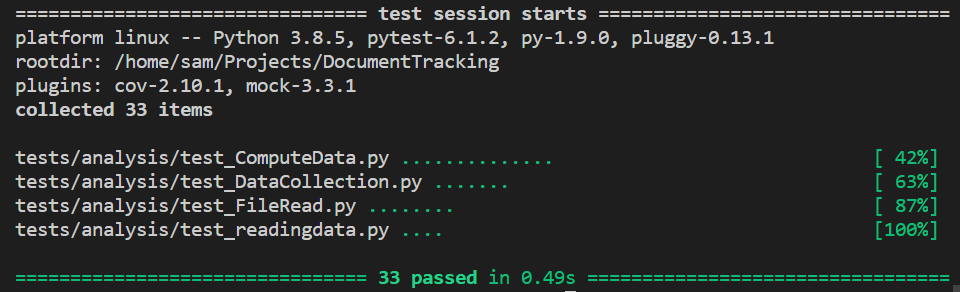
\includegraphics{pytest.png}
    \caption{Tests running and passing}
    \label{fig:pytest}
\end{figure}

The unit tests proved invaluable when working on the FileRead module with concurrency.
There are some issues with input validation handling logic, many possible CLI parameters have not been extensively tested so it may be possible to open the GUI without the requisite parameters. 

\section{Personal Development}
% ------------------------------------------- PERSONAL DEVELOPMENT ---------------------------------------------------------------
\emph{A short discussion on lessons learnt from the feedback given on CW1and a discussion how you integrated this feedback into CW2.  Cover both coding and report writing,possibly more (project management, preparing for interview style questions etc).}
Lessons learnt from the experience of CW1:
Started out using test driven development

\subsection{Code feedback}

\begin{itemize}
    \item Feedback: limited input validation - Considerably more input validation takes place, use of regex expressions and loops to allow users to re-enter data helps, however a more systematic approach would be better.
    \item Feedback: Too much global state, not restrictive access modifiers - This has laregely been addressed, but this is due to the language shift, python doesnt use public/private access modifiers.
    \item Feedback: No custom exceptions - Custom exceptions have been used for input validation, more custom exceptions could have been used but the descision was made to handle most exceptions right away using logic based around the \code{None} type (for the most part these are \code{KeyErrors}).
    \item Feedback: No checks for arguments - Pythons duck typing system can make resolving this more complicated, explicit primative type stubs (although not enforeced) should provide hints to other developers when debugging, also in some cases the \code{hasattr()} function was used to try and test the correct argument type was provided.
    \item Feedback: Too much code duplication - Some effort was made to reduce code duplication in the Gui by using methods to build repeated gui elements, there still exists some code duplication particularly in the DataCollector class. 
\end{itemize}

\subsection{Report feedback}
\begin{itemize}
    \item Introduction
        \begin{itemize}
            \item Feedback: Should briefly cover the spec - The introduction features a brief description of the spec.
            \item Feedback: Shoulc cover the goals - 
            \item Feedback: Discuss environment - Detail about the environment has been included in the introduction, from expected operating system to user technical competency and expected kind of hardware.
        \end{itemize}
    \item Developer guide
        \begin{itemize}
            \item Feedback: Discuss class dependencies - Class interdepenencies have been mentioned, additionally provided documenation supplies extra detail on this topic.
            \item Feedback: Discuss method interfaces - Some detail here, could include alot more but it feels somewhat redundant with the provided documentation and primative type stubs.
        \end{itemize}
    \item Conclusion
        \begin{itemize}
            \item Feeback: Should discuss advanced language features - 
        \end{itemize}
\end{itemize}


\section{Conclusions}
% ------------------------------------------- CONCLUSION ---------------------------------------------------------------
\emph{Reflect on what you are most proud of in the application and what you’d have likedto have done differently.  You should reflect on the produced software, and compare software devel-opment in scripting vs.  systems languages.}

Most proud of:
- Concurrency during file reading
- Structure of the code, good decoupling front and back end

Do differently:
- Leave more time to work on the gui
- Use a different library for the gui
- subclass the datacollector class to break it into smaller tasks




\pagebreak
\appendix
\section{References}
\printbibliography

\end{document}
